\documentclass[10pt,aspectratio=169]{beamer}

\usepackage{beamerthemeNAOCSlides}
\usepackage{amsmath,amssymb,booktabs,mathtools,array}
\usepackage{graphicx}
\usepackage{tikz}
\usetikzlibrary{arrows.meta,positioning,calc}

\graphicspath{{assets/}}

\definecolor{GateRed}{HTML}{C44E52}
\definecolor{GateBlue}{HTML}{2A579D}
\definecolor{GateGreen}{HTML}{1B7F5A}
\definecolor{GateGray}{HTML}{F4F6F8}
\newcommand{\code}[1]{\texttt{\detokenize{#1}}}
\newcommand{\yes}{\textcolor{GateGreen}{yes}}
\newcommand{\no}{\textcolor{GateRed}{no}}
\hypersetup{colorlinks=true,urlcolor=GateBlue,linkcolor=GateBlue}

\title{Pop II Top-heavy IMF Gate}
\subtitle{背景、方法、结果与文献依据}
\author{}
\institute{中国科学院国家天文台}
\date[2026-05-17]{2026-05-17}

\begin{document}

\NAOCTitlePage

\NAOCOutlinePage{
  \item 背景：为什么需要 source-time gate
  \item 方法：gate 判据与 UV convolution 实现
  \item 结果：Reed07 HMF + \(z=6\) calibration 后的 UVLF 响应
  \item 文献依据：top-heavy / FFB / rapid growth 的外部支撑
}

\NAOCSectionPage{Part.01}{背景}

\begin{NAOCBlankPage}{这件事到底在判断什么}
\begin{columns}[T,onlytextwidth]
  \column{0.50\textwidth}
  \begin{block}{判定对象}
    \begin{itemize}
      \item 判定单位是 Pop II 的 source-time SFR cell。
      \item Pop III 分支保持独立。
      \item Halo track 提供 \(M_{\rm h}(t')\)、\(\dot M_{\rm h}(t')\)、\(z(t')\)。
    \end{itemize}
  \end{block}

  \column{0.46\textwidth}
  \begin{block}{当前实现}
    \begin{itemize}
      \item 对每个 active cell 计算 \(I_{\rm TH}(t')\)。
      \item \(I_{\rm TH}=1\)：该时刻 SFR 选 mild top-heavy Pop II SSP。
      \item \(I_{\rm TH}=0\)：该时刻 SFR 选 canonical Pop II SSP。
    \end{itemize}
  \end{block}
\end{columns}

\vspace{0.45cm}
\centering
\begin{tikzpicture}[
  box/.style={draw=GateBlue,thick,rounded corners=3pt,fill=NAOCLight,
    minimum width=2.65cm,minimum height=0.72cm,align=center},
  gate/.style={draw=GateGreen,thick,rounded corners=3pt,fill=GateGray,
    minimum width=2.95cm,minimum height=0.72cm,align=center},
  arr/.style={-{Latex[length=2.2mm]},thick,draw=GateBlue}
]
  \node[box] (mah) {MAH + SFR history};
  \node[gate,right=0.65cm of mah] (flag) {\(I_{\rm TH}(t')\)};
  \node[box,right=0.65cm of flag] (ssp) {SSP kernel choice};
  \node[box,right=0.65cm of ssp] (uvlf) {UVLF};
  \draw[arr] (mah) -- (flag);
  \draw[arr] (flag) -- (ssp);
  \draw[arr] (ssp) -- (uvlf);
\end{tikzpicture}
\end{NAOCBlankPage}

\NAOCSectionPage{Part.02}{方法}

\begin{NAOCBlankPage}{Gate 插入在 UV convolution 里}
\begin{columns}[T,onlytextwidth]
  \column{0.50\textwidth}
  \begin{block}{canonical component}
  \[
    L_{\rm can}=\int (1-I_{\rm TH})\,{\rm SFR}(t')\,
    \Psi_{\rm can}(t_{\rm obs}-t')\,dt'
  \]
  \end{block}

  \column{0.50\textwidth}
  \begin{block}{top-heavy component}
  \[
    L_{\rm TH}=\int I_{\rm TH}\,{\rm SFR}(t')\,
    \Psi_{\rm TH}(t_{\rm obs}-t')\,dt'
  \]
  \end{block}
\end{columns}

\vspace{0.35cm}
\begin{itemize}
  \item 总 UV 光度写成 \(L_{\rm UV}=L_{\rm can}+L_{\rm TH}\)。
  \item MAH、SFR efficiency、dust mapping 保持一致；只切换 UV convolution 里的 SSP kernel。
  \item 因此它是一个受控的 SSP sensitivity test；自洽 variable-IMF galaxy model 另行处理。
\end{itemize}
\end{NAOCBlankPage}

\begin{NAOCBlankPage}{三个 mode 的严格条件}
\small
\begin{center}
\begin{tabular}{p{0.25\linewidth}p{0.39\linewidth}p{0.25\linewidth}}
\toprule
Mode & 判断条件 & 物理含义 \\
\midrule
\code{canonical} &
\(I_{\rm TH}(t')=0\) &
永远不触发 top-heavy \\
\code{z10_mild_topheavy} &
\(I_{\rm TH}(t')=\mathbf{1}[z(t')\ge z_{\rm TH}]\) &
\(z_{\rm TH}=10\) 以上 source time 全部切换 \\
\code{mah_burst_mild_topheavy} &
\(\mathbf{1}[z(t')\ge z_{\rm TH}]\,\mathbf{1}[\tau_{\rm grow}(t')\le\tau_{\rm th}]\) &
只保留高红移且快速增长的子集 \\
\bottomrule
\end{tabular}
\end{center}

\vspace{0.3cm}
\begin{columns}[T,onlytextwidth]
  \column{0.48\textwidth}
  \begin{block}{默认阈值}
  \[
    z_{\rm TH}=10,\qquad \tau_{\rm th}=50~{\rm Myr}
  \]
  \end{block}

  \column{0.48\textwidth}
  \begin{block}{MAH growth time}
  \[
    \tau_{\rm grow}(t')=\frac{M_{\rm h}(t')}{\dot M_{\rm h}(t')}
  \]
  代码里只接受有限、正的 \(M_{\rm h}\) 和 \(\dot M_{\rm h}\)。
  \end{block}
\end{columns}
\end{NAOCBlankPage}

\begin{NAOCBlankPage}{代码里是哪一段在判定}
\scriptsize
\begin{center}
\begin{tabular}{p{0.24\linewidth}p{0.27\linewidth}p{0.41\linewidth}}
\toprule
位置 & 关键对象 & 作用 \\
\midrule
\code{auroralf/uvlf/imf.py} &
\code{compute_topheavy_source_flags} &
mode + \(z(t')\) + \(M_{\rm h}/\dot M_{\rm h}\) + active mask \(\rightarrow I_{\rm TH}\)。 \\
\code{auroralf/uvlf/pipeline.py} &
\code{starforming_grid}, \code{topheavy_source_grid} &
只在正在形成星的 source-time cell 上判断 gate。 \\
\code{auroralf/uvlf/pipeline.py} &
\(L_{\rm can}\), \(L_{\rm TH}\) &
canonical 与 top-heavy SSP 分别卷积，再相加。 \\
\code{auroralf/uvlf/hmf_sampling.py} &
sample weights &
Reed07 HMF 权重进入 UVLF histogram。 \\
\bottomrule
\end{tabular}
\end{center}

\vspace{0.18cm}
\footnotesize
\textbf{一句话：} top-heavy 的“哪部分”就是 \code{topheavy_source_grid=True} 的 source-time SFR；halo track 和 UVLF 只在之后聚合。
\end{NAOCBlankPage}

\begin{NAOCBlankPage}{判断流程}
\small
\begin{center}
\begin{tabular}{p{0.16\linewidth}p{0.38\linewidth}p{0.32\linewidth}}
\toprule
Step & 条件 & 结果 \\
\midrule
1 & SFR cell 不 active & canonical SSP \\
2 & mode 是 \code{canonical} & canonical SSP \\
3 & \(z(t')<10\) & canonical SSP \\
4a & \code{z10_mild_topheavy} 且 \(z(t')\ge10\) & top-heavy SSP \\
4b & \code{mah_burst_mild_topheavy} 且 \(z(t')\ge10\)，\(\tau_{\rm grow}\le50~{\rm Myr}\) & top-heavy SSP \\
4c & \code{mah_burst_mild_topheavy} 但 \(\tau_{\rm grow}>50~{\rm Myr}\) & canonical SSP \\
\bottomrule
\end{tabular}
\end{center}

\vspace{0.25cm}
\begin{block}{最关键的一行}
\[
I_{\rm TH}^{\rm MAH}(t')=
\mathbf{1}\!\left[z(t')\ge10\right]\,
\mathbf{1}\!\left[\frac{M_{\rm h}(t')}{\dot M_{\rm h}(t')}\le50~{\rm Myr}\right].
\]
\end{block}
\end{NAOCBlankPage}

\NAOCSectionPage{Part.03}{结果与结论}

\begin{NAOCBlankPage}{HMF 与 \(z=6\) 校准}
\begin{columns}[T,onlytextwidth]
  \column{0.48\textwidth}
  \begin{block}{本版计算设置}
  \begin{itemize}
    \item HMF：\code{hmf} package 的 Reed07 fitting function。
    \item redshift：\(z=6,\,12.5,\,14.5\)。
    \item dust：统一用同一套 \(M_{\rm UV}^{\rm int}\rightarrow M_{\rm UV}^{\rm obs}\) mapping。
  \end{itemize}
  \end{block}

  \column{0.48\textwidth}
  \begin{block}{只在 \(z=6\) 调 \(\epsilon_0\)}
  \[
    \epsilon_0=0.10212
  \]
  \small
  由 \(z=6\) UVLF detections 的 log-space residual 标定；之后固定该值预测高红移。
  \end{block}
\end{columns}

\vspace{0.30cm}
\begin{block}{为什么要重做}
从历史 ST / massfunc HMF 换到 Reed07 后，\(z=6\) canonical UVLF 的归一化改变；不能沿用旧 \(\epsilon_0\) 直接读 top-heavy 响应。
\end{block}
\end{NAOCBlankPage}

\begin{NAOCBlankPage}{Gated UVLF result}
\centering
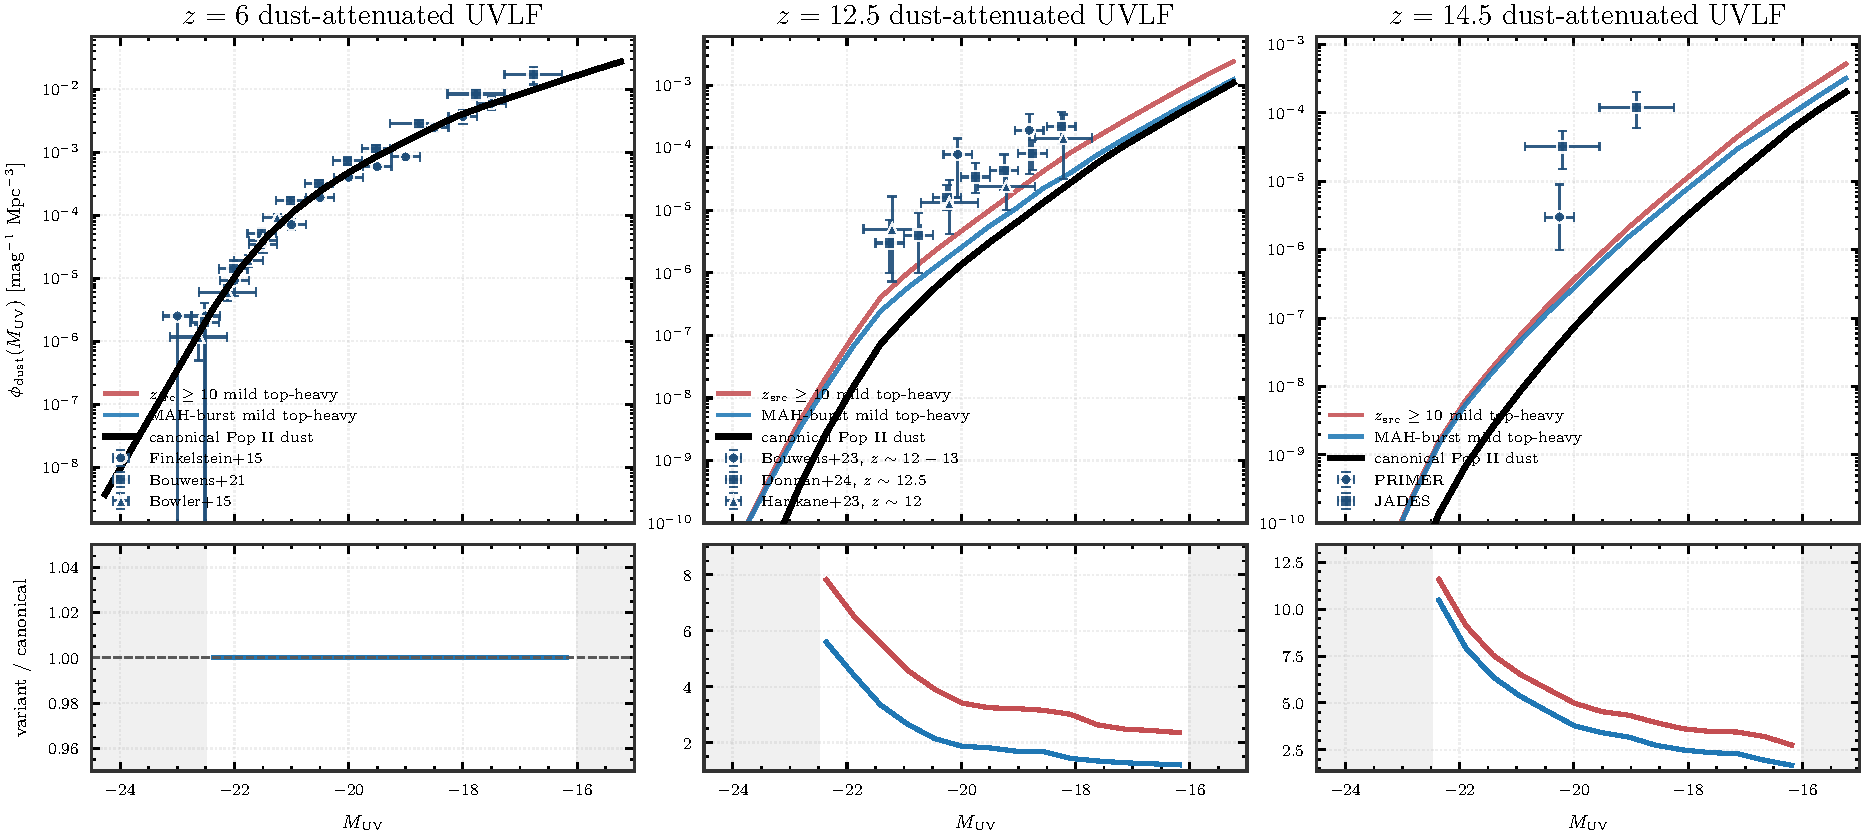
\includegraphics[height=0.80\textheight]{topheavy_uvlf_reed07_eps0p10212_z6_z12p5_z14p5.pdf}
\end{NAOCBlankPage}

\begin{NAOCBlankPage}{定量读数}
\footnotesize
\begin{center}
\begin{tabular}{lccp{0.33\linewidth}}
\toprule
Redshift / range & \(R_z=\phi_z/\phi_{\rm can}\) & \(R_{\rm MAH}=\phi_{\rm MAH}/\phi_{\rm can}\) & 解释 \\
\midrule
\(z=6\) & \(1.00\) & \(1.00\) & calibration unchanged \\
\(z=12.5\), full & \(3.34\) & \(1.85\) & bright-end sensitive \\
\(z=12.5\), obs range & \(3.24\) & \(1.76\) & \(-22.5\le M_{\rm UV}\le -16\) \\
\(z=14.5\), obs range & \(4.44\) & \(3.30\) & higher rapid-growth fraction \\
\bottomrule
\end{tabular}
\end{center}

\vspace{0.35cm}
\begin{block}{结论}
\(z\)-gate 给出上限响应；MAH gate 把 top-heavy 限制在 rapid-growth source-time 子集，因此更保守。
\end{block}
\end{NAOCBlankPage}

\begin{NAOCBlankPage}{边界条件：保持哪些量固定}
\begin{columns}[T,onlytextwidth]
  \column{0.48\textwidth}
  \begin{block}{保持固定}
  \begin{itemize}
    \item \(\epsilon_0\) 只由 \(z=6\) 标定一次；高红移固定。
    \item SN feedback / gas recycling 固定。
    \item metal enrichment 与 dust production 固定。
    \item inferred stellar mass comparison 固定。
  \end{itemize}
  \end{block}

  \column{0.48\textwidth}
  \begin{block}{应该怎么表述}
  canonical Pop II 是 fiducial；两个 mild top-heavy mode 是文献动机下的 sensitivity mapping。
  \end{block}
  \begin{block}{表达边界}
  避免把 MAH gate 说成自洽的气体密度、金属丰度或局域 SFH model；它只是 source-time proxy。
  \end{block}
\end{columns}
\end{NAOCBlankPage}

\begin{NAOCBlankPage}{最后要讲清楚的三句话}
\begin{enumerate}
  \item Top-heavy 的对象是 Pop II source-time SFR cell；halo track 与 Pop III 保持独立。
  \item 判断条件只有两层：\(z_{\rm src}\ge10\)，以及可选的 \(\tau_{\rm grow}=M_{\rm h}/\dot M_{\rm h}\le50~{\rm Myr}\)。
  \item Reed07 HMF 下，\(z=6\) 标定 \(\epsilon_0=0.10212\)；\(z=12.5\) 观测相关区间中，\(z\)-gate 约 \(3.24\)，MAH gate 约 \(1.76\)。
\end{enumerate}
\end{NAOCBlankPage}

\NAOCSectionPage{Part.04}{文献依据}

\begin{NAOCBlankPage}{文献依据 1：top-heavy IMF 与高 SFR/吸积环境}
\centering
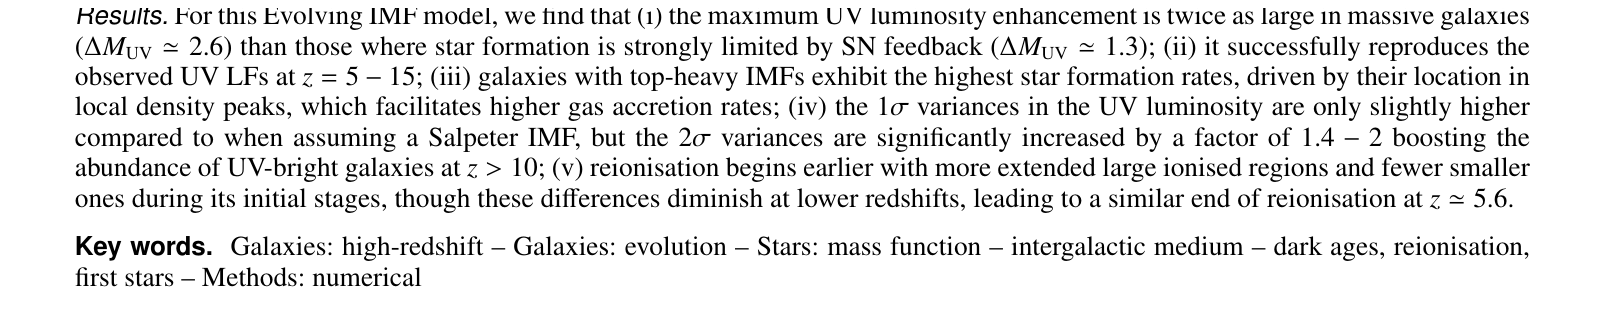
\includegraphics[width=0.94\linewidth]{lit_hutter2025_results_excerpt.png}
\vspace{0.12cm}

{\small \href{https://arxiv.org/pdf/2410.00730\#page=1}{Hutter et al. 2025, A\&A / arXiv:2410.00730, p.1}}
\vspace{0.20cm}

\begin{columns}[T,onlytextwidth]
  \column{0.31\textwidth}
  \begin{block}{UV 增亮}
    \small \(\Delta M_{\rm UV}\simeq2.6\) in massive galaxies。
  \end{block}
  \column{0.31\textwidth}
  \begin{block}{环境}
    \small highest SFR；local density peaks。
  \end{block}
  \column{0.31\textwidth}
  \begin{block}{吸积}
    \small higher gas-accretion rates。
  \end{block}
\end{columns}
\end{NAOCBlankPage}

\begin{NAOCBlankPage}{文献依据 2：为什么 MAH growth 可以当 proxy}
\centering
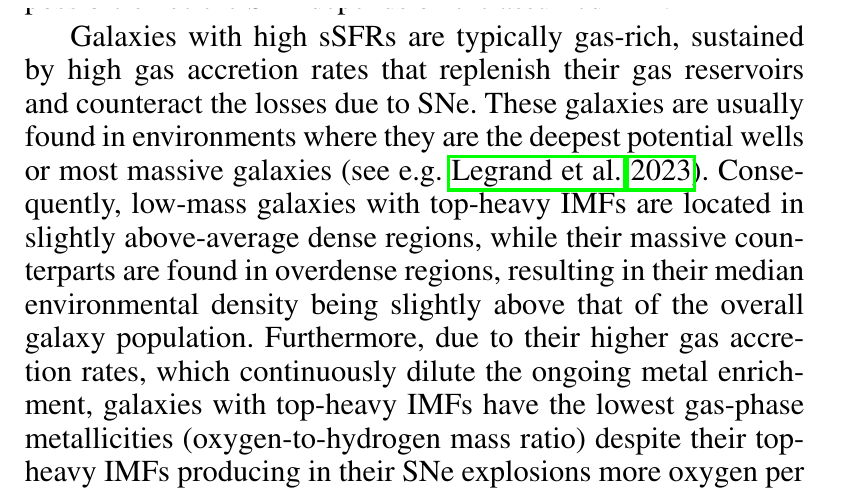
\includegraphics[width=0.65\linewidth]{lit_hutter2025_gas_accretion.png}
\vspace{0.12cm}

{\small \href{https://arxiv.org/pdf/2410.00730\#page=8}{Hutter et al. 2025, Section 5, p.8}}
\vspace{0.06cm}

{\small \textbf{Gate：} high gas accretion / rapid growth \(\Rightarrow\tau_{\rm grow}\) proxy}
\end{NAOCBlankPage}

\begin{NAOCBlankPage}{文献依据 3：FFB abstract 的直接依据}
\centering
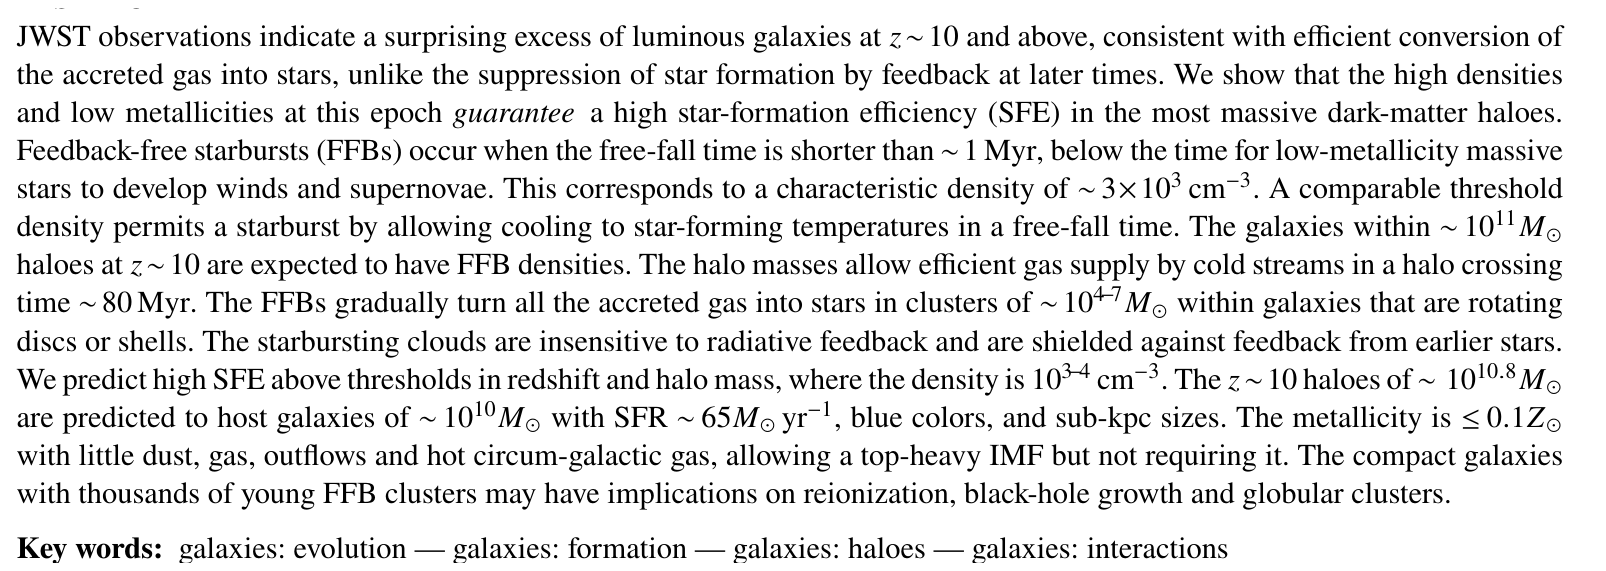
\includegraphics[width=0.90\linewidth]{lit_dekel2023_abstract_excerpt.png}
\vspace{0.15cm}

{\small \href{https://arxiv.org/pdf/2303.04827\#page=1}{Dekel et al. 2023, MNRAS / arXiv:2303.04827, p.1}}
\vspace{0.12cm}

\begin{minipage}{0.90\linewidth}
\small
\textbf{抽取数字：} \(t_{\rm ff}\lesssim1~{\rm Myr}\), \(n\sim10^3\)--\(10^4~{\rm cm^{-3}}\), halo crossing \(\sim80~{\rm Myr}\)，并说明 top-heavy IMF is allowed but not required。
\end{minipage}
\end{NAOCBlankPage}

\begin{NAOCBlankPage}{文献依据 4：FFB 的图像化时标}
\begin{columns}[T,onlytextwidth]
  \column{0.46\textwidth}
  \centering
  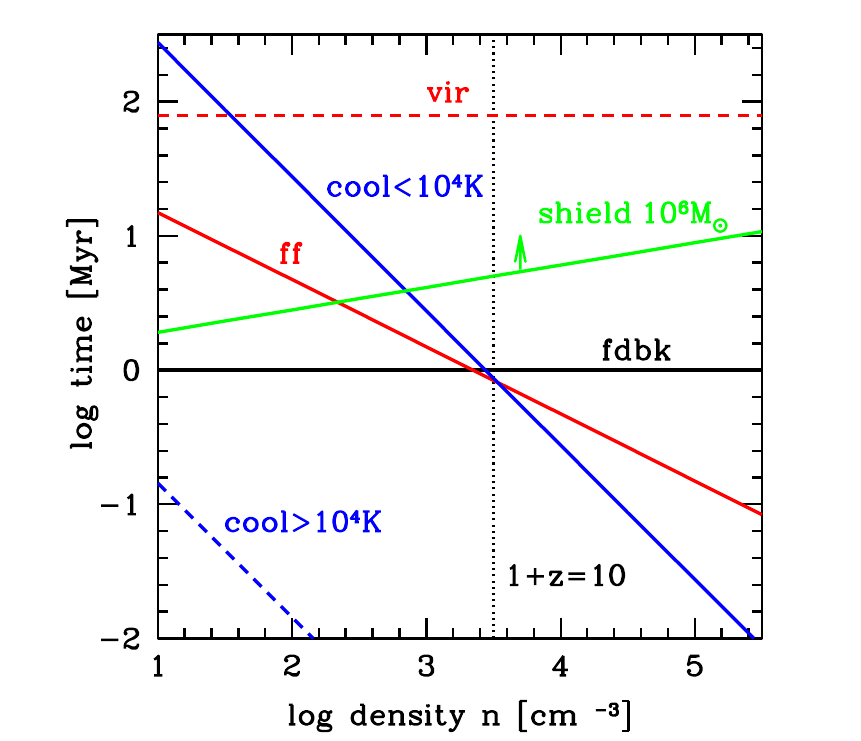
\includegraphics[height=0.70\textheight]{lit_dekel2023_timescale_fig_only.png}

  \column{0.50\textwidth}
  \begin{block}{Dekel et al. 2023 给出的图像}
    \begin{itemize}
      \item feedback-free burst 需要 \(t_{\rm ff}\lesssim1~{\rm Myr}\)。
      \item 对应 characteristic density 约 \(10^{3}\)--\(10^{4}\,{\rm cm^{-3}}\)。
      \item halo crossing/gas supply 是更长的 \(\sim80~{\rm Myr}\) 量级。
    \end{itemize}
  \end{block}
  \vspace{0.15cm}
  {\small \href{https://arxiv.org/pdf/2303.04827\#page=5}{Dekel et al. 2023, Fig. 3, p.5}}
\end{columns}
\end{NAOCBlankPage}

\begin{NAOCBlankPage}{文献依据 5a：FFB phase 与 10 Myr burstiness}
\centering
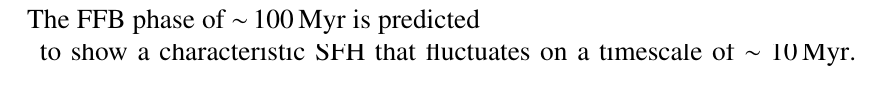
\includegraphics[width=0.84\linewidth]{lit_li2024_100myr_zoom.png}
\vspace{0.12cm}

{\small \href{https://arxiv.org/pdf/2311.14662\#page=1}{Li et al. 2024, A\&A / arXiv:2311.14662, p.1}}
\vspace{0.16cm}

\begin{minipage}{0.88\linewidth}
\small
\textbf{取值含义：} FFB phase \(\sim100~{\rm Myr}\)，characteristic SFH fluctuation \(\sim10~{\rm Myr}\)；我们的 \(50~{\rm Myr}\) 是 rapid-growth cut，物理 burst duration 需要另行建模。
\end{minipage}
\end{NAOCBlankPage}

\begin{NAOCBlankPage}{文献依据 5b：bursty SFH 的图像证据}
\begin{columns}[T,onlytextwidth]
  \column{0.58\textwidth}
  \centering
  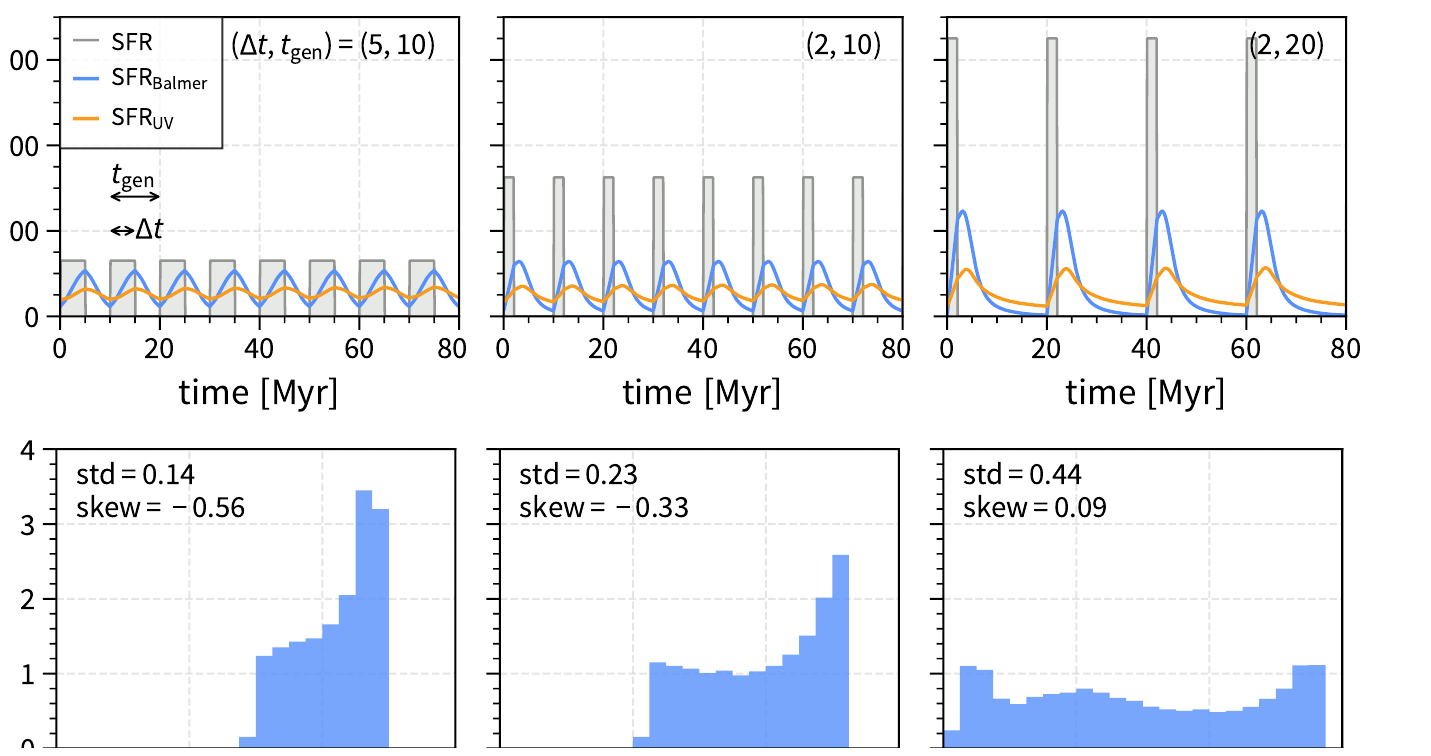
\includegraphics[width=\linewidth]{lit_li2024_bursty_sfh_panels.png}
  \vspace{0.10cm}

  {\small \href{https://arxiv.org/pdf/2311.14662\#page=9}{Li et al. 2024, Fig. 9, p.9}}

  \column{0.38\textwidth}
  \begin{block}{映射到 gate}
  \begin{itemize}
    \item 图中 SFH 是 \(\sim10~{\rm Myr}\) fluctuation。
    \item \(50~{\rm Myr}\) 只筛 rapid-growth source time。
    \item 它比 \(\sim80\)--\(100~{\rm Myr}\) 供气/FFB 阶段更保守。
  \end{itemize}
  \end{block}
\end{columns}
\end{NAOCBlankPage}

\begin{NAOCBlankPage}{把文献映射回我们的 gate}
\scriptsize
\begin{center}
\begin{tabular}{p{0.27\linewidth}p{0.35\linewidth}p{0.26\linewidth}}
\toprule
文献图像 & 放进模型的 proxy & 对应 mode \\
\midrule
\(z>10\) UV-bright tension &
\(z_{\rm src}\ge10\) &
\code{z10_mild_topheavy} \\
highest SFR / gas-rich / high accretion &
\(\tau_{\rm grow}=M_{\rm h}/\dot M_{\rm h}\le50~{\rm Myr}\) &
\code{mah_burst_mild_topheavy} \\
FFB phase \(\sim80\)--\(100~{\rm Myr}\), bursty SFH \(\sim10~{\rm Myr}\) &
50 Myr rapid-growth cut; not burst duration &
保守限制 bright-end 响应 \\
\bottomrule
\end{tabular}
\end{center}

\vspace{0.25cm}
\begin{block}{讲的时候要强调}
这是 literature-motivated source-time proxy；它只标记 source-time 子集，不把所有 \(z>10\) Pop II 统一设为 top-heavy，也不把 MAH gate 等同于 gas density 或 metallicity model。
\end{block}
\end{NAOCBlankPage}

\begin{NAOCBlankPage}{文献链接（点击跳转）}
\footnotesize
\begin{itemize}
  \item \href{https://arxiv.org/pdf/2410.00730\#page=1}{Hutter et al. 2025, p.1: abstract results; top-heavy IMF, UV boost, density peaks, gas accretion}
  \item \href{https://arxiv.org/pdf/2410.00730\#page=8}{Hutter et al. 2025, p.8: high-sSFR / gas-rich / high-accretion environment}
  \item \href{https://arxiv.org/pdf/2303.04827\#page=1}{Dekel et al. 2023, p.1: FFB abstract; \(1~{\rm Myr}\), \(10^3\)--\(10^4~{\rm cm^{-3}}\), \(80~{\rm Myr}\)}
  \item \href{https://arxiv.org/pdf/2303.04827\#page=5}{Dekel et al. 2023, p.5: timescale-density Fig. 3}
  \item \href{https://arxiv.org/pdf/2311.14662\#page=1}{Li et al. 2024, p.1: FFB phase \(\sim100~{\rm Myr}\), SFH fluctuation \(\sim10~{\rm Myr}\)}
  \item \href{https://arxiv.org/pdf/2311.14662\#page=9}{Li et al. 2024, p.9: bursty SFH Fig. 9}
\end{itemize}

\vspace{0.18cm}
\begin{block}{备注}
这些链接是外部 PDF 页码锚点；大多数 PDF viewer / browser 会直接跳到对应页。
\end{block}
\end{NAOCBlankPage}

\NAOCThanksPage

\end{document}
